\chapter{Функции обработчика прерывания от системного таймера}

\section{UNIX}

\subsection*{По тику:}

\begin{itemize}[label=---]
\item инкремент счетчика реального времени;
\item инкремент счетчика времени, прошедшего с момента запуска системы;
\item инкремент счетчика процессорного времени, полученного текущим
процессором в режиме задачи и в режиме ядра;
\item декремент счетчиков времени, оставшегося до отправления на выполнение отложенных вызовов, при достижении нулевого значения счетчиков выставление флага, указывающего на необходимость запуска обработчика отложенного вызова
\item декремент кванта.
\end{itemize}

\subsection*{По главному тику:}

\begin{itemize}[label=---]
\item выполнение связанных с планированием процессов, например пересчет приоритетов и проверку истечения временного кванта для процесса;
\item пробуждение (регистрация отложенного вызова процедуры $wakeup$, которая перемещает дескриптор процесса из списка «спящих» в очередь «готовых к выполнению») системных процессов, таких как $swapper$ и $pagedaemon$;
\item декремент счетчика времени, оставшегося до посылки одного из следующих сигналов: 
\begin{itemize}[label=---]
    \item \texttt{SIGALRM} --- сигнал посылается процессу по истечении времени, которое было предварительно задано через системный вызов alarm;
    \item \texttt{SIGPROF} --- сигнал, посылаемый процессу по истечению времени, заданного в таймере профилирования;
    \item \texttt{SIGVTALRM} --- сигнал, посылаемый процессу по истечении времени, заданного с помощью системного вызова setitimer.
\end{itemize}
\end{itemize}

\subsection*{По кванту:}

\begin{itemize}
\item посылка сигнала \texttt{SIGXCPU} активному процессу, если тот превысил выделенный для него квант процессорного времени~\cite{unix}.
\end{itemize}

\section{Windows}

\subsection*{По тику:}

\begin{itemize}[label=---]
\item инкремент счетчика реального времени;
\item декремент счетчика времени отложенных задач;
\item декремент кванта.
\end{itemize}

\subsection*{По главному тику:}

\begin{itemize}[label=---]
\item Инициализация диспетчера настройки баланса путем сбрасывания объекта <<событие>>, на котором он ожидает (диспетчер настройки баланса по событию от таймера сканирует очередь готовых процессов и повышает приоритет процессов, которые находились в очереди в состоянии ожидания дольше 4х секунд).
\end{itemize}

\subsection*{По кванту:}

\begin{itemize}[label=---]
	\item инициализирует диспетчеризацию потоков с добавлением соответствующего объекта в очередь DPC~\cite{win}.
\end{itemize}

\chapter{Пересчет динамических приоритетов}

\section{UNIX}

Планирование процессов в UNIX основано на приоритете процессов. Каждый процесс обладает приоритетом планирования, изменяющимся с течением времени. Планировщик всегда выбирает процесс с наивысшим приоритетом. Для диспетчеризации процессов с равным приоритетом применяется вытесняющее квантование времени. Изменение приоритетов процессов происходит динамически на основе количества используемого ими процессорного времени. Необходимо проводить пересчет приоритетов, чтобы исключить бесконечное откладывание.

Традиционное ядро UNIX является строго невытесняющим, однако в современных системах UNIX ядро является вытесняющим -- то есть процесс в режиме ядра может быть вытеснет более приоритетным процессом в режиме ядра. Ядро сделано вытесняющим для того, чтобы система могла обслуживать такие процессы, как процессы на звуковой карте. 

В операционных системах Unix был введен механизм многозадачности,
при котором один процесс может включать несколько параллельно выполняющихся потоков. Эти потоки разделяют адресное пространство и другие ресурсы процесса, но выполняются независимо друг от друга. Каждый поток имеет свой контекст, который включает в себя регистры и стек, специфичные для его выполнения. Однако общие для всех потоков ресурсы остаются
в контексте самого процесса.

Приоритет процесса задается любым целым числом, которое лежит в диапазоне от 0 до 127 (чем меньше число, тем выше приоритет)
\begin{enumerate}
	\item 0 - 49 -- зарезервированы для ядра (приоритеты ядра статические)
	\item 50 - 127 -- прикладные процессы (приоритеты прикладных процессов динамические, т.е. могут изменяться во времени)
\end{enumerate}

Структура \texttt{proc}, представляющая собой дескриптор процесса, содержит следующие поля, относящиеся к приоритетам:
\begin{enumerate}
	\item \texttt{p\_pri} -- текущий приоритет планирования;
	\item \texttt{p\_usrpri} -- приоритет режима задачи;
	\item \texttt{p\_cpu} -- результат последнего измерения использования процессора;
	\item \texttt{p\_nice} -- фактор <<любезности>>, который устанавливается пользователем.
\end{enumerate}

Планировщик использует \texttt{р\_рri} для принятия решения о том, какой процесс направить на выполнение. \texttt{p\_pri} и \texttt{p\_usrpri} равны, когда процесс находится в режиме задачи.

Значение \texttt{p\_pri} может быть изменено (повышено) планировщиком для того, чтобы выполнить процесс в режиме ядра. В таком случае \texttt{p\_usrpri} будет использоваться для хранения приоритета, который будет назначен процессу, когда тот вернется в режим задачи.

\texttt{p\_cpu} инициализируется нулем при создании процесса (и на каждом тике обработчик таймера увеличивает это поле текущего процесса на 1, до максимального значения равного 127).

Ядро системы связывает приоритет сна с событием или ожидаемым ресурсом, из-за которого процесс может блокироваться (приоритет сна определяется для ядра, поэтому лежит в диапазоне 0--49). Когда процесс <<просыпается>>, ядро устанавливает \texttt{p\_pri}, равное приоритету сна события или ресурса, по которому произошла блокировка (значение приоритета сна для некоторых событий в системе 4.3BSD представлены в таблице \ref{tab:bsd}).


\begin{table}[h!]
	\caption{Приоритеты сна в ОС \texttt{4.3BSD}}
	\label{tab:bsd}
		\begin{tabularx}{\textwidth}{|c|c|X|}
			\hline
			\textit{Приоритет} & \textit{Значение} & \textit{Описание} \\
			\hline
			\texttt{PSWP} & 0 & Свопинг \\
			\hline
			\texttt{PSWP + 1} & 1 & Страничный демон \\
			\hline
			\texttt{PSWP + 1/2/4} & 1/2/4 & Другие действия по обработке памяти \\
			\hline
			\texttt{PINOD} & 10 & Ожидание освобождения inode \\
			\hline
			\texttt{PRIBIO} & 20 & Ожидание дискового ввода-вывода \\
			\hline
			\texttt{PRIBIO + 1} & 21 & Ожидание освобождения буфера \\
			\hline
			\texttt{PZERO} & 25 & Базовый приоритет \\
			\hline
			\texttt{TTIPRI} & 28 & Ожидание ввода с терминала \\
			\hline
			\texttt{TTOPRI} & 29 & Ожидание вывода с терминала \\
			\hline 
			\texttt{PWAIT} & 30 & Ожидание завершения процесса потомка \\
			\hline
			\texttt{PLOCK} & 35 & Консультативное ожидание блок. ресурса \\
			\hline
			\texttt{PSLEP} & 40 & Ожидание сигнала \\
			\hline
		\end{tabularx}
\end{table}

Каждую секунду ядро системы инициализирует отложенный вызов процедуры \texttt{schedcpu()}, которая уменьшает значение \texttt{p\_pri} каждого процесса исходя из фактора <<полураспада>> (в системе 4.3BSD считается по формуле \ref{eq:ref1})

\begin{equation}
\label{eq:ref1}
decay = \frac{2 \cdot load\_average}{2 \cdot load\_average + 1},
\end{equation}

где
\textit{load\_average} --- это среднее количество процессов, находящихся в состоянии готовности к выполнению, за последнюю секунду.

Также процедура \texttt{schedcpu()} пересчитывает приоритеты для режима задачи
всех процессов по формуле \ref{eq:ref2},

\begin{equation}
\label{eq:ref2}
\texttt{p\_usrpri} = \texttt{PUSER} + \frac{\texttt{p\_cpu}}{2} + 2 \cdot \texttt{p\_nice},
\end{equation}

где \texttt{PUSER} --- базовый приоритет в режиме задачи, равный 50~\cite{unix}.

Таким образом, если процесс в последний раз использовал большое количество процессорного времени, то его \texttt{р\_срu} будет увеличен => рост значения \texttt{p\_usrpri} => понижение приоритета.  Чем дольше процесс простаивает в очереди на выполнение, тем больше фактор полураспада уменьшает его \texttt{р\_срu} => повышение его приоритета. Такая схема предотвращает бесконечное откладывание низкоприоритетных процессов. Применение данной схемы предпочтительно процессам, осуществляющим много операций ввода-вывода, в противоположность процессам, производящим много вычислений. То есть динамический пересчет приоритетов процессов в режиме задачи позволяет избежать бесконечного откладывания.

\section{Windows}
В ОС семейства Windows  процессу при создании назначается базовый приоритет. Относительно
базового приоритета процесса потоку назначается относительный приоритет. Планирование осуществляется на основе приоритетов потоков, готовых к выполнению. Поток с более низким приоритетом 
вытесняется потоком с более высоким приоритетом,в тот момент когда этот поток становится готовым к выполнению. По истечении кванта времени, выделенного 
текущему потока, ресурс передается самому приоритетному потоку в очереди готовых к выполнению. Каждый поток имеет динамический приоритет. Это приоритет, который планировщик использует для определения того, какой поток следует 
выполнить. Изначально динамический приоритет потока совпадает с базовым приоритетом процесса.

В ОС семейства Windows используется 32 уровня приоритета:
\begin{enumerate}
	\item от 0 до 15 --- динамические (изменяющиеся) уровни, при этом уровень 0 зарезервирован для потока обнуления страниц;
	\item от 16 до 31 --- статические уровни приоритета реального времени.
\end{enumerate} 

Динамический приоритет потока может временно повышаться или понижаться диспетчером планирования, чтобы улучшить отклик системы и обеспечить справедливое распределение процессорного времени. Однако система применяет такие корректировки только к потокам с базовым (статическим) приоритетом в диапазоне 0–15. Потоки с базовым приоритетом 16–31 считаются статическими: их приоритет не изменяется во время выполнения и используется исключительно для задач реального времени.

Уровни приоритета потоков назначаются с двух позиций: Windows API и ядра операционной системы. Windows API сортирует процессы по классам 
приоритета, которые были назначены при их создании:
\begin{itemize}
	\item Реального времени -- Real-time (4); 
	\item Высокий -- High (3);
	\item Выше обычного -- Above Normal (7);
	\item Обычный -- Normal (2);
	\item Ниже обычного -- Below Normal (5);
	\item Простоя -- Idle (1).
\end{itemize}

Затем назначается относительный приоритет потоков в рамках процес-
сов:
\begin{itemize}
	\item критичный по времени (time critical (15));
	\item наивысший (highest (2));
	\item выше обычного (above normal (1));
	\item ниже обычного (below normal (-1));
	\item обычный (normal (0));
	\item низший (lowest (-2));
	\item простой (idle (-15)).
\end{itemize}

Исходный базовый приоритет потока наследуется от базового приоритета процесса. Процесс по умолчанию наследует свой базовый приоритет у того 
процесса, который его создал.

Таким образом, в Windows API каждый поток имеет базовый приоритет, являющийся функцией класса приоритета процесса и его относительного 
приоритета процесса. В ядре класс приоритета процесса преобразуется в базовый приоритет. В таблице \ref{tbl:priority} приведено соответствие 
между приоритетами Windows API и ядра системы приоритета.

\begin{table}[H]
    \caption{Соответствие между приоритетами \textit{Windows API} и ядра Windows}
    \begin{center}
        \begin{tabularx}{\textwidth}{|l|X|X|X|X|X|X|}
            \hline
            {} & \textit{real-time} & \textit{high} & \textit{above normal} & \textit{normal} & \textit{below normal} & \textit{idle}\\
            \hline
            \textit{time critical} & 31 & 15 & 15 & 15 & 15 & 15 \\
            \hline
            \textit{highest} & 26 & 15 & 12 & 10 & 8 & 6 \\
            \hline
            \textit{above normal} & 25 & 14 & 11 & 9 & 7 & 5 \\
            \hline
            \textit{normal} & 24 & 13 & 10 & 8 & 6 & 4 \\
            \hline
            \textit{below normal} & 23 & 12 & 9 & 7 & 5 & 3 \\
            \hline
            \textit{lowest} & 22 & 11 & 8 & 6 & 4 & 2 \\
            \hline
            \textit{idle} & 16 & 1 & 1 & 1 & 1 & 1 \\
            \hline
        \end{tabularx}
    \end{center}
    \label{tbl:priority}
\end{table}

В Windows также включен диспетчер настройки баланса, который сканирует очередь готовых процессов 1 раз в секунду. 
Если он обнаруживает потоки, ожидающие выполнения более 4
секунд, диспетчер настройки баланса повышает их приоритет до 15. Когда истекает
квант, приоритет потока снижается до базового приоритета. Если поток не был завершен за квант времени или был вытеснен потоком с более высоким приоритетом, то
после снижения приоритета поток возвращается в очередь готовых потоков.

Текущий приоритет потока в динамическом диапазоне (от 1 до 15) может быть изменён планировщиком вследствие следующих причин:
\begin{itemize}
    \item повышение приоритета после завершения операций ввода-вывода;
    \item повышение приоритета владельца блокировки;
    \item повышение приоритета вследствие ввода из пользовательского интерфейса;
    \item повышение приоритета вследствие длительного ожидания ресурса исполняющей системы;
    \item повышение приоритета вследствие ожидания объекта ядра;
    \item повышение приоритета в случае, когда готовый к выполнению поток не был запущен в течение длительного времени;
    \item повышение приоритета проигрывания мультимедиа службой планировщика \textit{MMCSS}.
\end{itemize}

Кроме того, в различных заголовочных файлах Windows указаны рекомендуемые значения, которые следует использовать коду режима ядра при вызове таких функций, как \textit{KeSetEvent} и \textit{KeReleaseSemaphore}. Эти значения определены как \textit{EVENT\_INCREMENT} и \textit{MUTANT\_INCREMENT} соответственно. В заголовках они всегда задаются равными 1, поэтому можно считать, что большинство случаев повышения приоритета при завершении ожидания на таких объектах приводит к увеличению приоритета на единицу.

Текущий приоритет потока в динамическом диапазоне может быть понижен до базового путем вычитания всех его повышений. В таблице \ref{tab:io} приведены рекомендуемые значения повышения приоритета для устройств ввода-вывода.

\begin{table}[H]
    \caption{Рекомендуемые значения повышения приоритета.}
    \begin{center}
        \begin{tabularx}{\textwidth}{|X|l|}
            \hline
            \textit{Устройство} & \textit{Повышение приоритета} \\
            \hline
            Звуковая карта & 8 \\
            \hline
            Клавиатура, мышь & 6 \\
            \hline
            Сеть, почтовый слот, именованный канал, последовательный порт & 2 \\
            \hline
            Жесткий диск, привод компакт-дисков, параллельный порт, видеоустройство & 1 \\
            \hline
        \end{tabularx}
    \end{center}
    \label{tab:io}
\end{table}

Большинство описанных выше повышений приоритетов перестают действовать после завершения кванта или нескольких, выделенных процессу.
На рисунке~\ref{fig:priorgraph} представлен пример повышения и понижения приоритетов.

\begin{figure}[H]
	\centering
	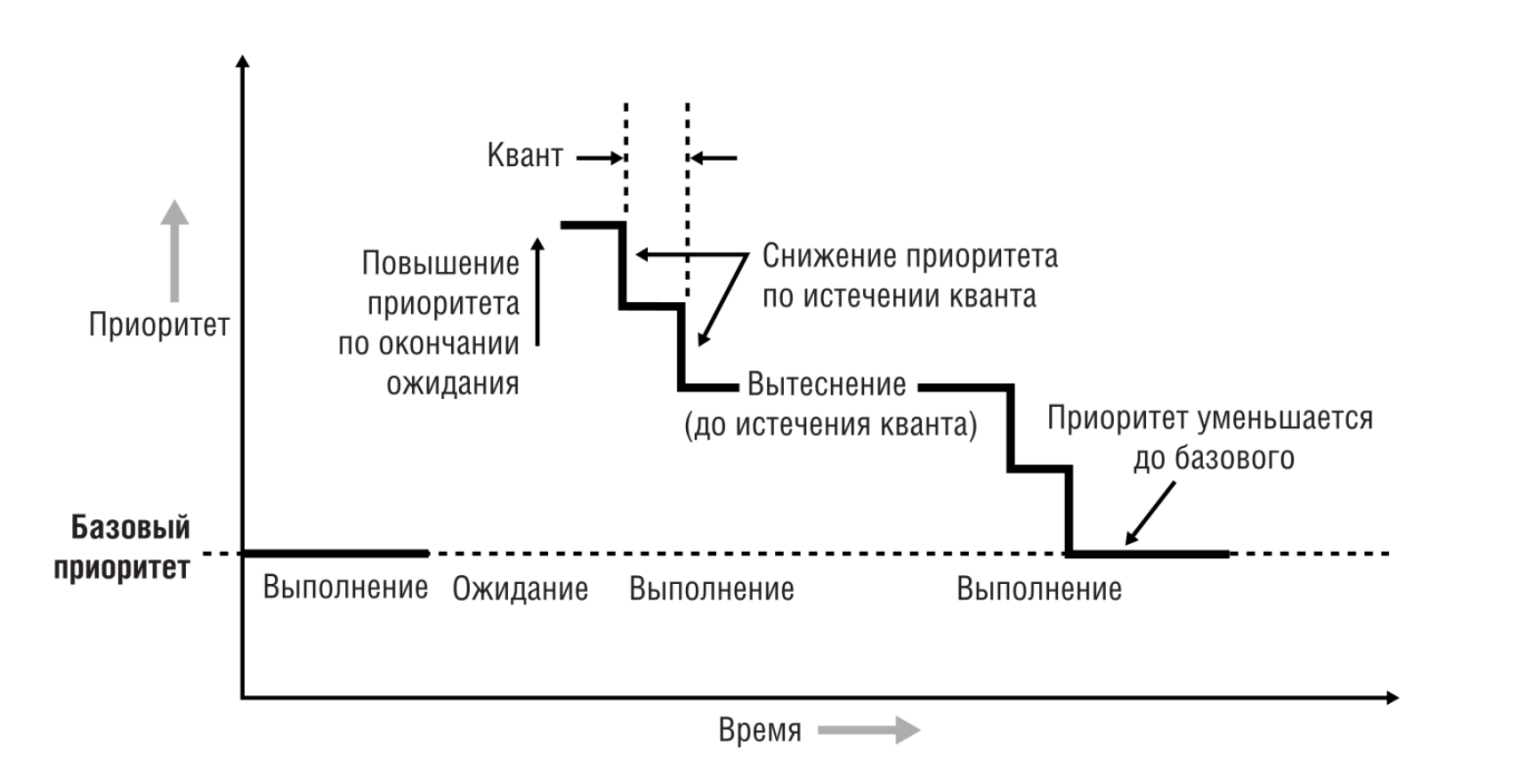
\includegraphics[width=0.6\textwidth]{images/image}
	\caption{Повышение и снижение приоритета}
	\label{fig:priorgraph}
\end{figure}


\textbf{MMCSS}
Потоки, на которых выполняются различные мультимедийные приложения, должны выполняться с минимальными задержками, причем выполнение потоков, работающих с аудио должно быть наиболее приоритетным, так как человеческий слух чувствителен к задержкам. В Windows эта задача решается путем повышения приоритетов таких потоков драйвером \texttt{MMCSS} --- MultiMedia Class Scheduler Service.

Одно из наиболее важных свойств для планирования потоков --- категория планирования --- первичный фактор определяющий приоритет потоков, зарегистрированных в \texttt{MMCSS}. Различные категории планирования представлены в таблице \ref{tab:plan}.

\begin{table}[H]
	\caption{Категории планирования.}
	\begin{center}
		\begin{tabularx}{\textwidth}{|p{42mm}|p{28mm}|X|}
			\hline
			\textbf{Категория} & \textbf{Приоритет} & \textbf{Описание} \\
			\hline
			High (Высокая) & 23-26 & Потоки, связанные с обработкой аудио , работают с более высоким приоритетом, чем большинство потоков в системе, за исключением потоков, обеспечивающих выполнение критически важных системных задач. \\
			\hline
			Medium (Средняя) & 16-22 & Потоки, поддерживающие выполнение активных приложений, например, таких как Windows Media Player, имеют умеренный приоритет. \\
			\hline
			Low (Низкая) & 8-15 & Потоки, не относящиеся к приложениям первого плана или задачам повышенного приоритета, выполняются с обычным уровнем приоритета. \\
			\hline
			Exhausted (Исчерпавших потоков) & 1-7 & Потоки, использовавшие своё доступное время на процессоре, продолжают выполнение только тогда, когда потоки с более высоким приоритетом не готовы к работе. \\
			\hline
		\end{tabularx}
	\end{center}
	\label{tab:plan}
\end{table}


Функции драйвера MMCSS временно повышают приоритет потоков, зарегистрированных с
MMCSS до уровня, который соответствует категории планирования. Потом их приоритет снижается до уровня, соответствующего категории планирования Exhausted, для
того, чтобы другие потоки тоже могли получить ресурс.

\textbf{IRQL}

Контроллеры прерываний сами устанавливают приоритетность своих прерываний, однако Windows определяет свою схему приоритетности, называемую IRQL, которая представлена на рисунке~\ref{fig:IRQL}.

\begin{figure}[H]
	\centering
	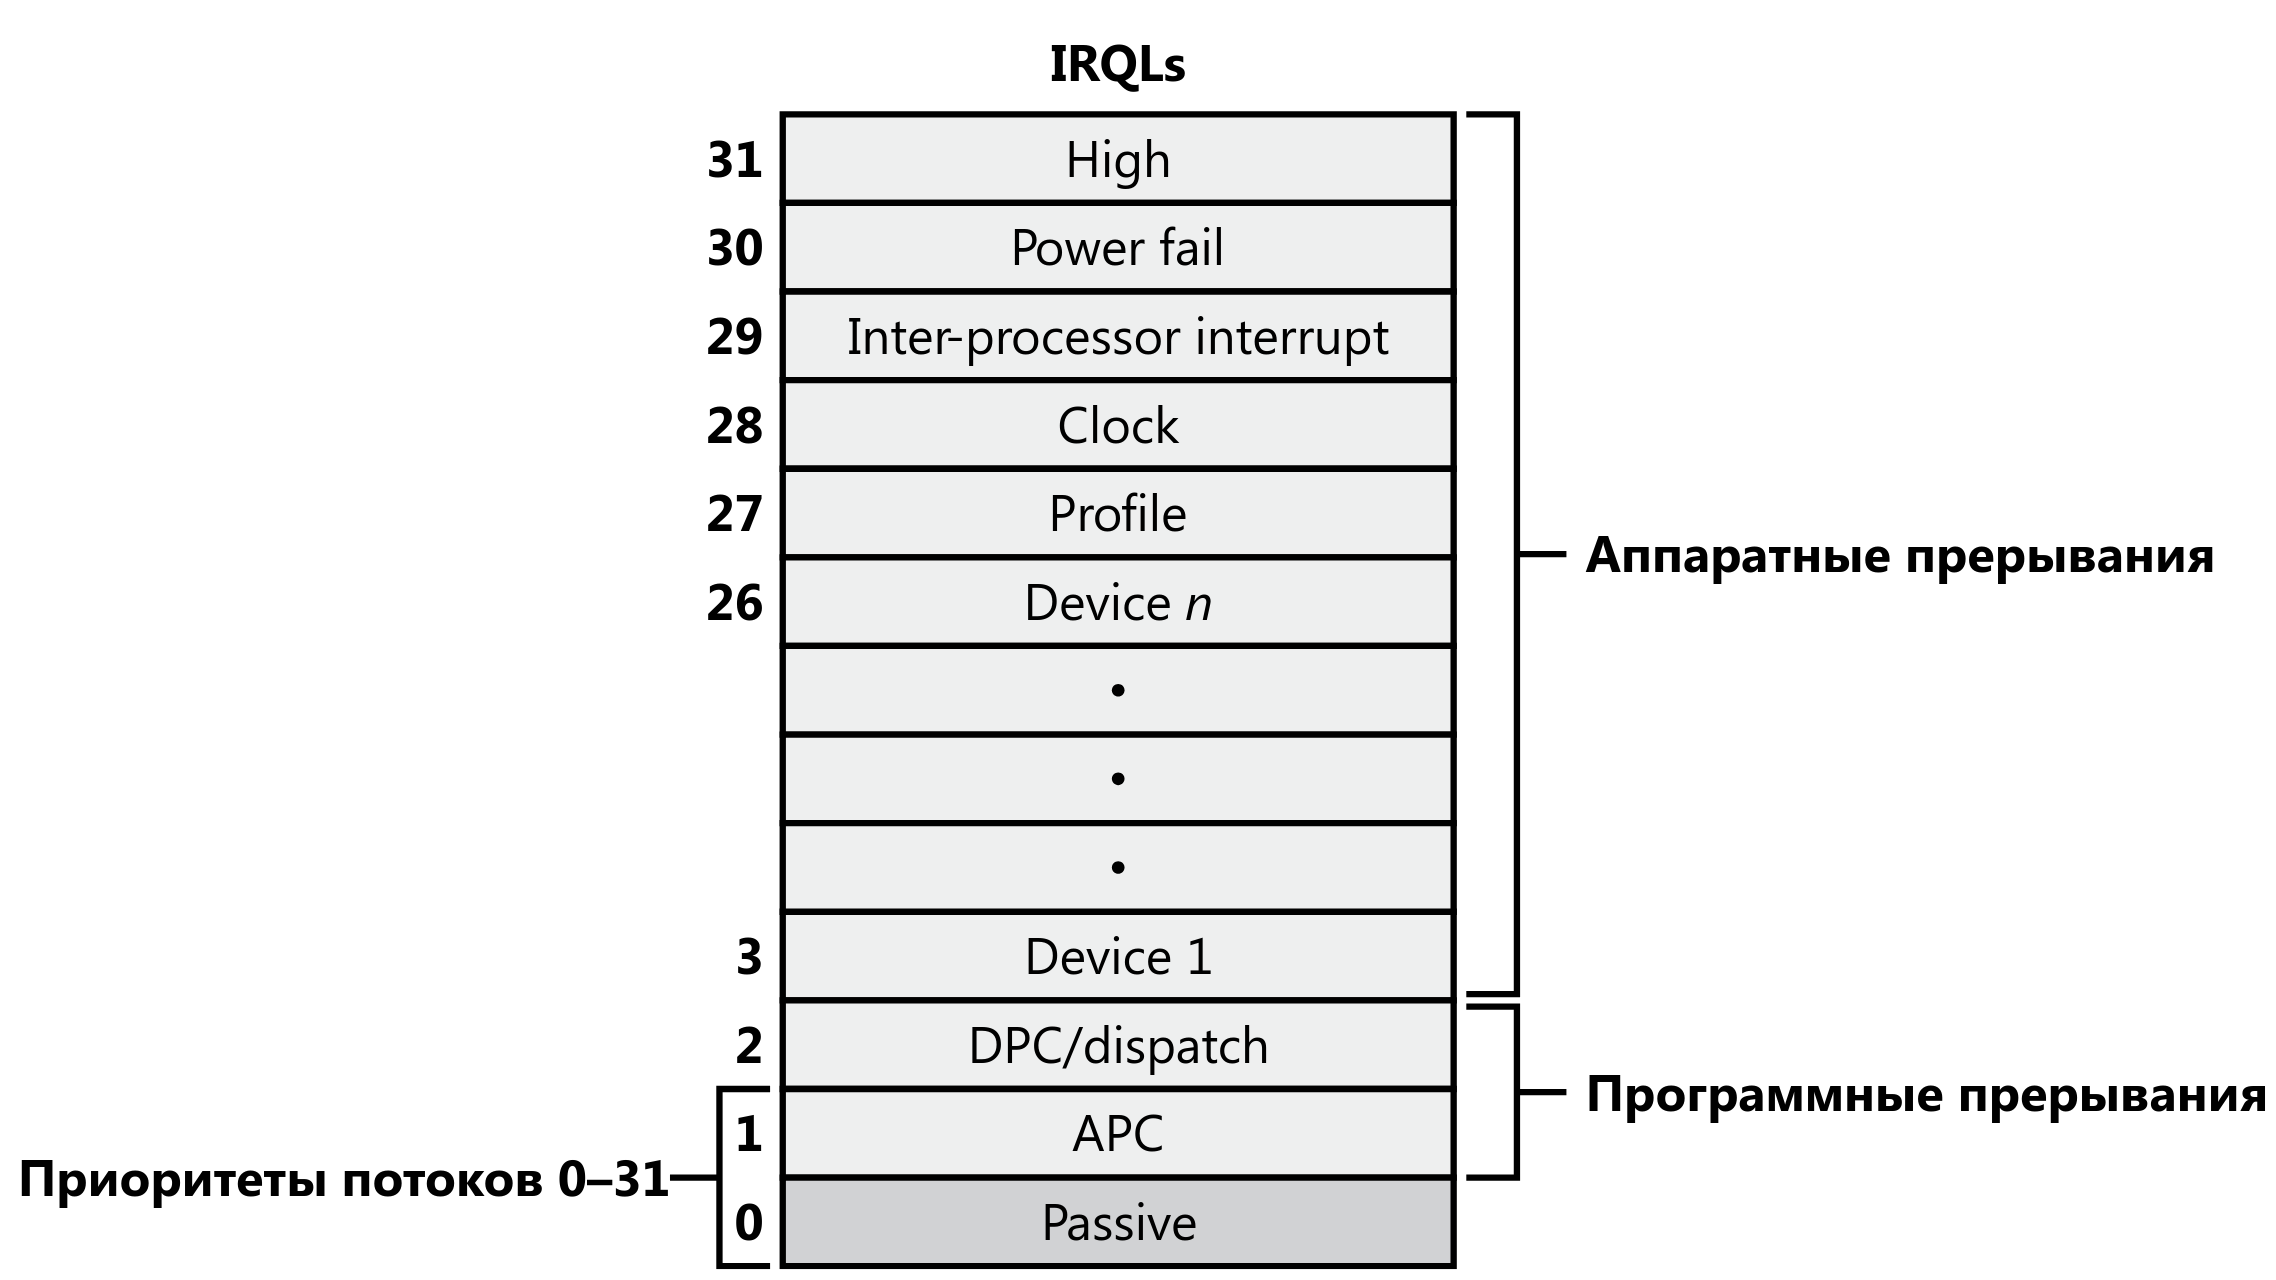
\includegraphics[width=0.8\textwidth]{images/IRQL}
	\caption{Сопоставление приоритетов потоков с IRQL-уровнями на системе x86}
	\label{fig:IRQL}
\end{figure}

Потоки обычно запускаются на уровне IRQL 0 или на уровне IRQL 1 (APC-уровень). Код пользовательского режима всегда запускается на пассивном уровне. Поэтому никакие потоки пользовательского уровня независимо от их приоритета не могут даже заблокировать аппаратные прерывания.

Потоки, запущенные в режиме ядра, несмотря на изначальное планирование на пассивном уровне или уровне APC, могут поднять IRQL на более высокие уровни, например, при выполнении системного вызова, который может включать в себя диспетчеризацию потока, диспетчеризацию памяти или ввод-вывод. Если поток поднимает IRQL на уровень dispatch или еще выше, на его процессоре не будет больше происходить ничего, относящегося к планированию потоков, пока уровень IRQL не будет опущен ниже уровня dispatch, так как прерывания обрабатываются в порядке из приоритетности. Поток выполняется на dispatch-уровне и выше, блокирует активность планировщика потоков и мешает контекстному переключению на своем процессоре.